\begin{frame}\frametitle{\vspace*{0.5cm}I plan to increase the relevance to DUS}
  Hypothesis: Baroclinic vorticity drives deformation to the point of
  stress or strain failure in pulmonary capillaries.
  % 
  \begin{itemize}
  \item Rabbit pulmonary capillaries have been shown to hemorrhage at transmural stresses of $\approx 5$ kPa \citep{West1991}.
  \item I will calculate elastic and (passive) viscous stresses at the interface.\vfill%
    \vspace*{5pt}
  \end{itemize}
  % 
  \begin{figure}
    \centering
    \def\svgwidth{0.4\textwidth}%
    {\tiny
      \import{./figs/}{usbe_lung_model_arclength.pdf_tex}%
    }
  \end{figure}
  %
  \note{
    \footnotesize{
      \begin{enumerate}
      \item I hypothesize that vorticity induced elastic or viscous
        stress could be resulting in hemorrhage of the fragile
        alveolar walls and the pulmonary capillaries within.
      \item To test this, I'm going to calculate the strain of the
        interface based on it's arclength as a function of time, and
        use this with the elastic modulus of lung tissue to see if the
        stresses that occur are high enough to be in expected failure
        regime for alveoli and pulmonary capillaries.
      \item Similarly, I'm going to use the velocity gradients in the
        measured flows to compute the (passive) viscous shear stress
        fields and compare to accepted failure stresses.
      \end{enumerate}
    }
  }
\end{frame}

\begin{frame}\frametitle{\vspace*{0.5cm}I plan to increase the relevance to DUS}
  Hypothesis: vorticity induced deformation and subsequent hemorrhage will allow acoustic waves and hemorrhage to propagate into
  subsequent layers of alveoli\\
  \begin{itemize}
  \item Damage exists in clearly defined hemorrhage area, not behind it \citep{Penney1993a}.
  \item Propagation mechanism of US-induced lesions are unknown \citep{Zachary2006}.
  \end{itemize}
  \begin{figure}
    \centering
    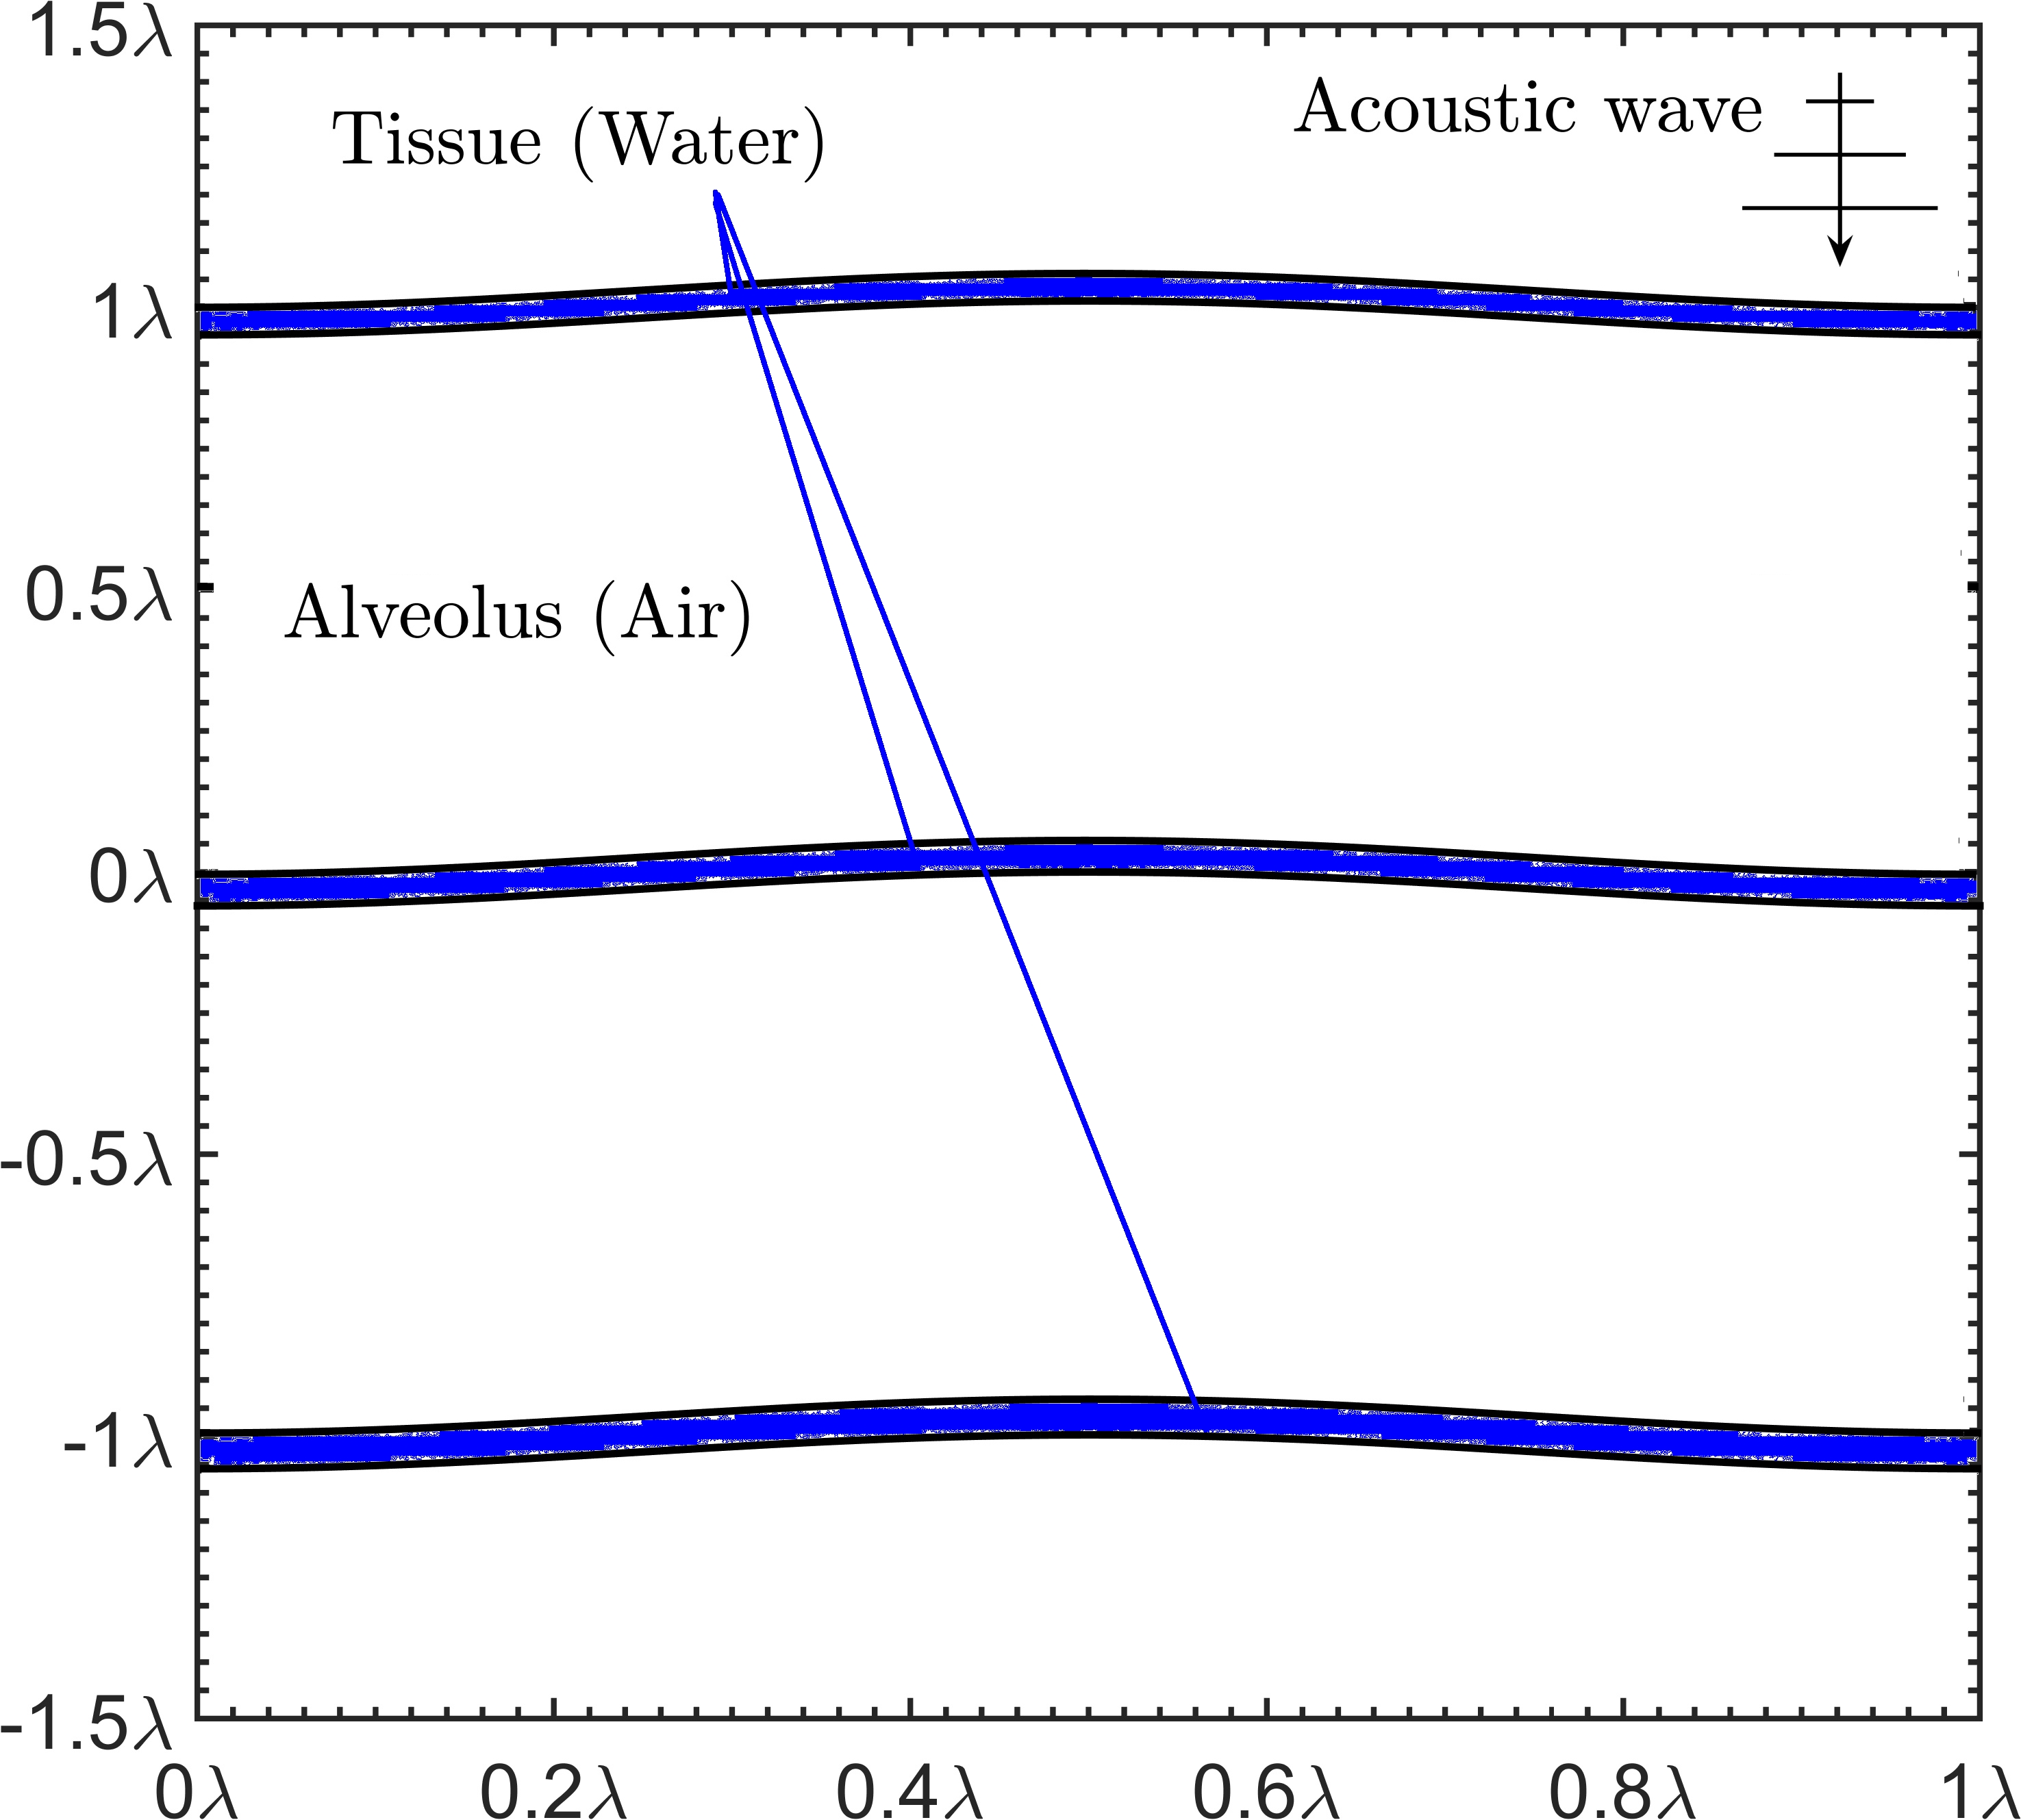
\includegraphics[width=0.5\textwidth]{../figs/lung_figs/usbe_model_schematic_periodic}
  \end{figure}
    \note{
    \footnotesize{
      \begin{enumerate}
      \item I also hypothesize that this mechanism will help explain
        how acoustic waves and hemorrhage propagate into subsequent
        layers of alveoli.
      \item To qualitatively test this, I plan to thin subsequent
        water layers in between air layers after each alveolar length
        scale.
      \item This will allow me to simulate how liquid might penetrate
        into an alveolus after a single ultrasound pulse, such that
        the next pulse could penetrate deeper, effecting adjacent
        alveoli.
      \item Quantitatively, this could also be used to estimate a
        hemorrhage propagation rate if the expected alveolar
        penetration times are short relative to the time between
        subsequent pulses.
      \end{enumerate}
    }
  }
  % \note{Mauro's Question:
  %   (1) Would a bubble-like configuration be more relevant/useful?
  % }
\end{frame}

\begin{frame}\frametitle{Future work (beyond me)}
  To fully understand the role that fluid mechanics plays in DUS-induced lung hemorrhage, the following problems need to be addressed:\\
  \vspace*{0.25cm}
  \begin{itemize}
  \item Viscous effects\vfill%
  \item Elasticity and failure mechanics\vfill%
  \item Multiple pulses (via time-dependent boundary conditions)\vfill%
  \item Detailed pulmonary structure\vfill%
  \end{itemize}
\end{frame}
%
%%% Local Variables:
%%% mode: latex
%%% TeX-master: "../main"
%%% End:
